\documentclass[UTF8,11pt,a4paper,fontset=fandol]{ctexart}

\usepackage[margin=22mm]{geometry}
\usepackage{amsmath,amssymb,booktabs,array,tabularx,longtable}
\usepackage{tikz,pgfplots,xcolor,enumitem,fancyhdr,hyperref}
\pgfplotsset{compat=1.18}
\definecolor{deepblue}{HTML}{267E9A}
\definecolor{warmred}{HTML}{CD715C}
\definecolor{slate}{HTML}{6A7B8C}
\definecolor{lavender}{HTML}{A494B8}
\hypersetup{colorlinks=true,linkcolor=deepblue,citecolor=deepblue,urlcolor=deepblue}
\setlength{\headheight}{15pt}
\pagestyle{fancy}\fancyhf{}\fancyhead[L]{\small NN-native current design: Stage 0}\fancyhead[R]{\small 3 October 2026}\fancyfoot[C]{\thepage}
\setlength{\parskip}{5pt}
\setlength{\emergencystretch}{2em}
\newcommand{\norm}[1]{\left\lVert #1\right\rVert}
\newcommand{\R}{\mathbb{R}}
\newcommand{\C}{\mathbb{C}}
\newcommand{\Id}{\mathrm{Id}}
\newcommand{\op}[1]{\operatorname{#1}}
\newcommand{\Cov}{\operatorname{Cov}_{12}}
\newcommand{\code}[1]{\texttt{#1}}
\newcommand{\coverageTable}{
\begin{center}\small\begin{tabular}{lrrrrr}\toprule
Method & smooth & near-contact & layered & asymmetric & Mean\\\midrule
B0 & 0.9689 & 0.3528 & 0.9198 & 0.6589 & 0.7251 \\
B1 ($s=02$) & 0.9317 & 0.5809 & 0.9010 & 0.7647 & 0.7946 \\
B1 ($s=03$) & 0.9658 & 0.8326 & 0.3139 & 0.8541 & 0.7416 \\
B1 ($s=04$) & 0.9760 & 0.5426 & 0.9379 & 0.9287 & 0.8463 \\
B2 & 0.9718 & 0.5178 & 0.9852 & 0.6751 & 0.7875 \\
B3 & 0.7283 & 0.4142 & 0.7644 & 0.5969 & 0.6259 \\
B4 & 1.0000 & 1.0000 & 1.0000 & 1.0000 & 1.0000 \\
B5 & 1.0000 & 1.0000 & 1.0000 & 1.0000 & 1.0000 \\
\bottomrule\end{tabular}\end{center}}
\newcommand{\coverageFig}{
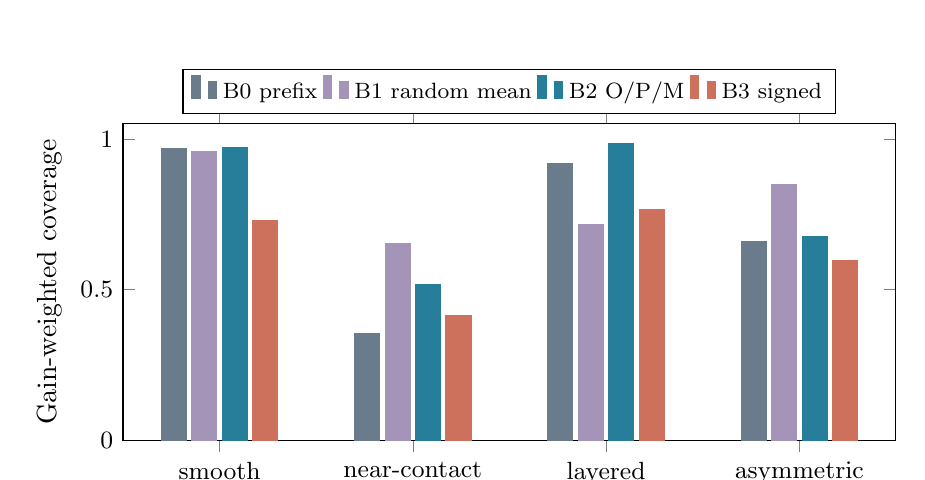
\begin{tikzpicture}\begin{axis}[width=.94\linewidth,height=5.6cm,ybar,bar width=9pt,ymin=0,ymax=1.05,xmin=-.5,xmax=3.5,
xtick={0,1,2,3},xticklabels={smooth,near-contact,layered,asymmetric},ylabel={Gain-weighted coverage},
legend style={at={(.5,1.03)},anchor=south,legend columns=4,font=\footnotesize},tick label style={font=\small}]
\addplot[fill=slate,draw=slate] coordinates {(0,0.96892621) (1,0.35281852) (2,0.91981014) (3,0.65892407)};
\addplot[fill=lavender,draw=lavender] coordinates {(0,0.95783071) (1,0.65206036) (2,0.71758396) (3,0.84914981)};
\addplot[fill=deepblue,draw=deepblue] coordinates {(0,0.97184706) (1,0.51782080) (2,0.98516681) (3,0.67505852)};
\addplot[fill=warmred,draw=warmred] coordinates {(0,0.72834963) (1,0.41419167) (2,0.76436052) (3,0.59686521)};
\legend{B0 prefix,B1 random mean,B2 O/P/M,B3 signed}
\end{axis}\end{tikzpicture}}
\newcommand{\marginFig}{
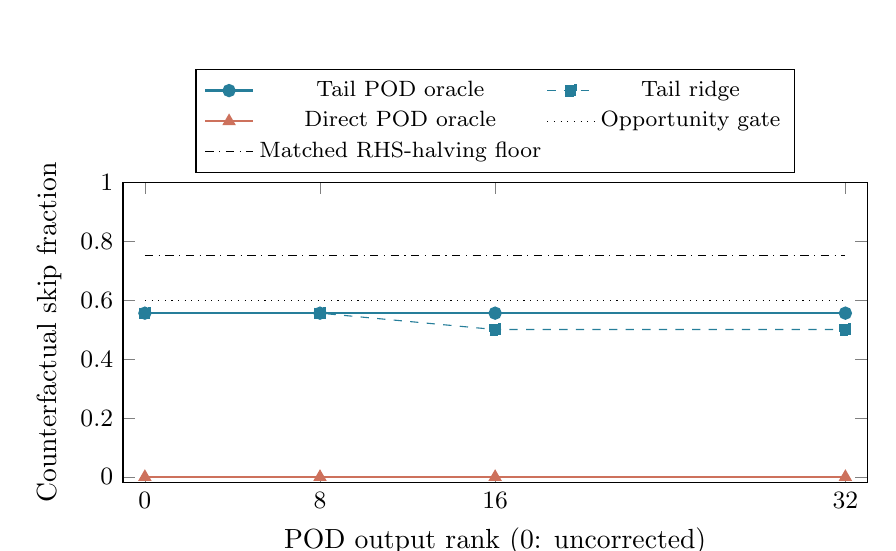
\begin{tikzpicture}\begin{axis}[width=.91\linewidth,height=5.4cm,xmin=-1,xmax=33,ymin=-.02,ymax=1,
xtick={0,8,16,32},xlabel={POD output rank (0: uncorrected)},ylabel={Counterfactual skip fraction},
legend style={at={(.5,1.03)},anchor=south,legend columns=2,font=\footnotesize},tick label style={font=\small}]
\addplot[deepblue,thick,mark=*] coordinates {(0,.55556)(8,.55556)(16,.55556)(32,.55556)};
\addplot[deepblue,dashed,mark=square*] coordinates {(0,.55556)(8,.55556)(16,.5)(32,.5)};
\addplot[warmred,thick,mark=triangle*] coordinates {(0,0)(8,0)(16,0)(32,0)};
\addplot[black,dotted,mark=none] coordinates {(0,.6)(32,.6)};
\addplot[black,dashdotted,mark=none] coordinates {(0,.75)(32,.75)};
\legend{Tail POD oracle,Tail ridge,Direct POD oracle,Opportunity gate,Matched RHS-halving floor}
\end{axis}\end{tikzpicture}}
\setlength{\parindent}{2em}

\title{NN-native Maxwell Current Design\\从问题、推导到本轮证据的完整讲解}
\author{中文研究稿理解与阅读指南}
\date{2026年10月3日}
\begin{document}\maketitle
\begin{abstract}
本讲解按英文研究稿的同一论证顺序，完整解释问题、物理接口、解析算法、实验结果和分支判断，再补充逐步推导及双语术语。读完后应能区分：候选覆盖与排序精度，measurement defect 与 full-current defect，representation oracle 与可部署 predictor，约60\%的历史机会门槛与本次75\%的成本门槛。实际结论是 A 建议下一阶段 tiny pilot；B 全范围数据不足，有完整 Gaussian 标签部分的当前正交主成分与固定 ridge 表示没有额外 margin/cost 空间。神经网络训练与新增物理 actions 均未启动。
\end{abstract}
\tableofcontents\clearpage

\section{英文研究稿的核心问题：NN 应学习什么}
\emph{Reduced current model（降阶电流模型）} 用少量电流方向替代高维 Maxwell current solve。\emph{Current dictionary（电流字典）} 是可以选取的原子集合；一个原子有固定的 physical ID。\emph{Incoming shortlist（候选短名单）} 先挑十二个未选原子，让后续昂贵端点评分仅在这十二个上进行。

这种设计的目标最终是 inverse problem 的 \emph{material update（材料更新）}。观测很强的 current，不一定能改善材料步；改动 current span，也不等于改动 material direction。英文稿第一个问题因此是：强的廉价物理筛选之后，learned candidate generator 还有多大可兑现的机会？第二个问题是：已存的 directional defect 能否被压缩到足够精度，从而有机会减少 gain verification？

此前 full-dictionary anchor 的排序很准，但 near-contact/asymmetric 的十二候选覆盖差。这给 A 提供了明确的切入点。B 是另一条独立方向，不能因为 A 有机会就自动训练 B。Stage0 的作用是先排除错误输入、非法 teacher、低秩误判和成本错觉。

\section{物理变量、共享材料 gauge 与三个接口}
\subsection{从 Maxwell tangent 到共享材料步}
设当前物理状态冻结。$L$ 是 Maxwell current operator，$S$ 将电流映射到测量，$B_p$ 是第 $p$ 个 illumination 下材料扰动到 current source 的 tangent map。六个 illumination 都作用在同一个材料扰动 $d$ 上。我们不是对每个 illumination 独立求一套材料未知量。

保存的 \emph{material gauge（材料坐标规约）} 是 exact physical orthonormal tangent。Gaussian 有27个 complex coordinates，实化后54维；voxel有1728个complex coordinates，实化后3456维。$\ell$、steps 与 basis fingerprint 必须一致，不能把同维度但不同 basis 的系数直接混用。$\Lambda=\lambda_{\rm total}I$ 是保存的 total quadratic regularization（总二次正则），包含 prior precision（先验精度）与 Levenberg--Marquardt（LM）damping。以smooth early为例，$\lambda_{\rm total}=10^{-5}+10^{-2}=0.01001$。Step 与 frozen gain 均保留这个总量；$\ell$ 是另一个保存的线性项。

材料 packing 为
\[
 d=\begin{bmatrix}\Re d_c\\\Im d_c\end{bmatrix},\quad
 d_c=d_{1:q}+i d_{q+1:2q}.
\]
数据则对每个 illumination 先存 $[\Re y_p;\Im y_p]$，再依次堆六个块。这给出 $6\times2\times128=1536$ real measurements。材料实化与数据堆叠是两件不同的事。

\subsection{公共投影并不等于完整物理算子}
完整 current 有5184行，保存的正交 embedding $Q$ 有128列。公共数据是
\[
 \widetilde L=Q^*LQ,\quad \widetilde S=SQ,\quad PB_p=Q^*B_p.
\]
它们可以给已有字典中的 reduced endpoint 算 response 和 GN step。即使能精确求 $\widetilde L^{-1}$，也只是在128维公共模型中求解，不能凭它生成 full-wave $J_Fd$。尤其是 $Q$ 外的 current 或 injection 分量没有因此被观测到。

Gauss--Newton（GN）在冻结状态中最小化 reduced quadratic。令 $J_U$ 为材料到 observation 的实 Jacobian（导数矩阵），公共 receiver step 为
\[
 x=-(J_U^TJ_U+\Lambda)^{-1}(J_U^Tr+\ell).
\]
信息按费用分为 F0 已有缓存、F1 廉价投影特征、F2 实际 child GN/完整 anchor score、F3 full-wave teacher/reference。三类接口据此分开：public/proposal 只接收 F0/F1；teacher 保存 incoming utility 或向量 target；evaluator 拥有完整 Jacobian、$Q_{\rm true}$、truth 与 reference step。F2 的 child material step/完整 anchor score 在 shortlist 之后才使用。Object ID、路径、几何类别和 seed 可以记录 provenance/split，却不能进入网络作为捷径。current-family 是原子物理生成来源的元数据，可以合法使用。

\section{核心推导一：两侧 defect 为什么成立}
假设完整物理 $L$ 可逆，且 compressed block 通过稳定性门槛。对当前 selected span 的正交 basis $U$，定义
\[
 A_U=U^*LU,\qquad R_U=UA_U^{-1}U^*.
\]
$R_U$ 是 Galerkin current response，而不是 Euclidean projector。只要 $A_U$ 稳定，$R_ULR_U=R_U$：
\[
 UA_U^{-1}U^*LU A_U^{-1}U^*=UA_U^{-1}A_UA_U^{-1}U^*=R_U.
\]
由此，右侧 injection defect 和左侧 observation defect 为
\[
 I_{U,p}=(I-LR_U)B_p,\qquad O_U=S(I-R_UL).
\]
展开双侧乘积：
\begin{align*}
 O_UL^{-1}I_{U,p}
 &=S(I-R_UL)L^{-1}(I-LR_U)B_p\\
 &=S(L^{-1}-R_U-R_U+R_ULR_U)B_p\\
 &=S(L^{-1}-R_U)B_p.
\end{align*}
右边就是 full 与 reduced observation tangent 的差。因此
\[
 J_F-J_U=\op{realify}\{O_UL^{-1}I_{U,p}\}_{p=1}^6.
\]
这个推导使用一般 complex $L$，没有把它假设成 Hermitian/SPD。它告诉我们遗漏误差同时受 source injection、full current feedback 和 observation dressing 控制。仅看原子的观测能量，可能漏掉材料扰动的注入方向和 current feedback。

这是原有 Galerkin/Schur 代数的解释，不被写成新增数学原创性。实际公共计算只拥有投影 maps；等式中的 full $L^{-1}$ 留在物理解释或 evaluator 概念层。

\section{核心推导二：one-swap 的 Schur transfer 与物理 ID}
删除一个原子后，剩余 span 记为 $V$，其 compressed operator 为 $A_V=V^*LV$。把 incoming bank 记为 $C$，原被删 bank 记为 $A$（这里 $A$ 表示一个 bank，和 richer anchor 的下标应按上下文区分）。在 $V$ 外表述 bank $Z$，定义
\begin{align*}
 \bar Z&=Z-VA_V^{-1}V^*LZ,\\
 \Gamma_Z&=Z^*L\bar Z,\\
 N_{Z,p}&=Z^*(B_p-LR_VB_p),\quad Y_Z=S\bar Z.
\end{align*}
消去 retained block 后，新增 transfer 是 $Y_Z\Gamma_Z^{-1}N_{Z,p}$。因此交换造成
\[
 J_{V+C}-J_{V+A}=\op{realify}\{Y_C\Gamma_C^{-1}N_{C,p}-Y_A\Gamma_A^{-1}N_{A,p}\}_p.
\]
这里能共用 retained factor，但 child step 仍要解同一 real material normal problem；不能把 current transfer 直接当作材料 gain。

动作身份始终是 original dictionary atom ID。SVD/QR 会旋转 basis，因此 ``删除第几列正交基'' 不等于 ``删除哪个 physical atom''。实际数据接口保存原始 selected IDs、drop/add IDs，置换存储后映射回它们。

若 bank 相位变换为 $Z'=ZE$，$E$ 是对角 unitary，则
\[
 N'=E^*N,\quad \Gamma'=E^*\Gamma E,\quad Y'=YE.
\]
因此 $Y'\Gamma'^{-1}N'=Y\Gamma^{-1}N$。这些是 \emph{phase covariance（相位协变）} 的具体规则，最终物理动作应 \emph{phase invariant（相位不变）}。普通 complex feature concatenation 不会自动满足它；future network 必须单独通过这些测试。

scalar $\gamma$ 的 usual condition number 总是1，不能用它辨别近奇异。我们记录 normalized $|\gamma|$、retained core 的 reciprocal condition 与实际 child/core gate；block $\Gamma$ 才有有意义的 condition number。稳定性阈值保持 $10^{-10}$，不能用 arbitrary jitter 换取 ``PASS''。

\section{共同 query、teacher 与四折怎么构造}
一个 query 的身份包括 object/state/pool、selected physical IDs、公共 $x$ hash、anchor hash、$\ell/\Lambda$、gauge 和 receiver/operator layout。early 的不同对象可能都从零 contrast 出发，如果只按 state hash 去重，会错误合并物理上下文。

每个 query 的完整 one-swap 字典是 $k(154-k)$。四对象各三 phase、$k=4,8,16$，给出
\[
 12[4(154-4)+8(154-8)+16(154-16)]=47712.
\]
实测 unique moves=47,712、feasible=43,108、unique incoming utilities=5208、duplicate=0。数值 floor、actual rank、core/child feasibility、最优 drop 的并列集合都保留。No-op 的 utility 是0；本轮36 queries 都有超过 floor 的正收益，所以 no-positive query 数为0。

incoming teacher 是所有合法 drop 中的最大正收益：
\[
 t_i(q)=\max(0,\max_{a\in U_q,\,\mathrm{feasible}}Q_{q,a,i}).
\]
它不是 ``每个 query 恰好一个正标签''；不同 incoming 可以同时有正 utility，最优 drop 也可以并列。

\begin{center}\small\begin{tabular}{clll}\toprule
Fold & Train objects & Validation & Test\\\midrule
0 & layered, asymmetric & near-contact & smooth\\
1 & smooth, asymmetric & layered & near-contact\\
2 & smooth, near-contact & asymmetric & layered\\
3 & near-contact, layered & smooth & asymmetric\\\bottomrule
\end{tabular}\end{center}
每折有18 train/9 validation/9 test queries。所有 phases、$k$、moves、augmentations 都随对象进入同一 partition。任何 RMS、POD 或超参数选择不能偷看 test。这个 benchmark 是 retrospective object holdout，并非全新盲采集的数据。

\section{A 的固定算法步骤与结果逐项解读}
\subsection{B0/B1：原前缀和公平随机对手}
B0 在 current-family 之间 round-robin，每个 family 按原始顺序取前缀，直到十二个。因此它不是强物理筛选。B1 先固定 B0 的 family counts，再在各 family 中随机选同样数量，seed 为20261002/03/04。全部 seed 都报告，不能事后按对象挑一个最优 seed。

\subsection{B2：三个物理轴的 union}
用整个 receiver $U$ 构造 $\bar c_i$ 与 dressed observation $Y_i$。O轴衡量归一化 dressed observation；P轴保留两个方向的 retained coupling；M轴用公共 receiver material step $x$ 检查 projected injection：
\begin{align*}
 O_i&=\norm{Y_i}^2/\norm{c_i}^2,\\
 P_i&=(\norm{U^*Lc_i}^2+\norm{c_i^*LU}^2)/\norm{c_i}^2,\\
 M_i&=\sum_p|c_i^*(I-LR_U)B_px|^2/(\norm{x}^2\norm{c_i}^2).
\end{align*}
三个列表分别降序排序。按O/P/M固定轮转，每次取列表中下一个尚未出现的原子；重复就跳过，直到十二个。score relative $10^{-12}$ 范围作为数值并列，按 original ID 定序。这套参数在首次 outcomes 前冻结，没有依据结果调权重。

\subsection{B3：有符号的 addition proxy 与 diversity}
记 $w_i=\op{realify}\{Y_i\gamma_i^{-1}n_{p,i}\}_p$，$u_A=r+J_Ax$。proxy 是
\[
 s_i=-u_A^Tw_i-\tfrac12\norm{w_i}^2.
\]
先在 query 内做 percentile rank，再贪心选最大
\[
 \op{ranknorm}(s_i)-0.25\max_{j\in P}\frac{|Y_i^*Y_j|^2}{\norm{Y_i}^2\norm{Y_j}^2}.
\]
这个 overlap penalty 避免候选观察方向过度相似。注意 $w_i$ 来自 receiver 的 $x$ 和 addition，不是 child 的 $d$，也没有删除一个 atom 后的真实 retained core。因此它是廉价 proxy，不是 actual one-swap gain。

\subsection{B4/B5：昂贵参照与覆盖指标}
B4 用已有完整 dictionary endpoint/anchor score 排序；B5用已有 full-objective one-swap teacher，包含 no-op。它们本轮都用 archive 查表，不能把查表速度算成真实 deploy speed。

\emph{Cov12（增益加权十二候选覆盖）} 是每个 query 池内最佳正gain的总和，除以完整字典最佳正gain总和。Top1 recall 检查是否捕获任何并列最优 incoming；top4 recall 是捕获的 tied top-four 集合比例；gain regret 是遗漏的gain。零分母应 NA，不能装成0或1。四对象mean等权，不让较大 objective scale 支配结论。

\coverageTable
\begin{figure}[htbp]\centering\coverageFig
\caption{覆盖图。B0复核历史瓶颈；B2对 near-contact/layered 有改善；B3没有把有符号 addition transfer 变成更好的材料动作。random均值不掩盖三个seed的完整表。}\end{figure}

\textbf{第一个发现：完整 anchor 排序够好，incoming pool 才是缺口。} B0分别为smooth 0.9689、near-contact 0.3528、layered 0.9198、asymmetric 0.6589；B4 anchor top1 capture 依次为0.9960、0.9810、0.9937、0.9883。仅提高排序并不能把未进入池子的 atom 变出来。

\textbf{第二个发现：廉价物理特征能改善，但没有关闭 opportunity。} B2把 near-contact 从0.3528提高到0.5178，把layered提高到0.9852，却仍失败于 near-contact0.70、asymmetric0.85、mean0.85三门槛。signed B3 的mean0.6259是需要保留的失败：更复杂的物理proxy不保证更好材料utility。

\textbf{第三个发现：随机 seed 的对象间不稳定，不能用事后 routing 虚构解析胜利。} seed03使near-contact达到0.8326、asymmetric0.8541，但layered只有0.3139；seed04mean0.8463，near-contact只有0.5426。单个固定cheap baseline到teacher的mean gap为0.1537。这提供 A 的试验价值，不保证NN能达到teacher。

下面表列出并列最优相关的recall和原始objective中的regret；完整三随机seed与每query记录在CSV。
\begin{center}\small\begin{tabular}{llrrr}\toprule Object & Method & Top1 & Top4 & Regret sum\\\midrule
smooth & B0 & 0.222 & 0.111 & 4.79e-05 \\
smooth & B2 & 0.222 & 0.167 & 4.34e-05 \\
smooth & B3 & 0.000 & 0.000 & 4.18e-04 \\
smooth & B4 & 1.000 & 1.000 & 0.00e+00 \\
near-contact & B0 & 0.000 & 0.000 & 1.94e-04 \\
near-contact & B2 & 0.111 & 0.083 & 1.45e-04 \\
near-contact & B3 & 0.000 & 0.028 & 1.76e-04 \\
near-contact & B4 & 1.000 & 1.000 & 0.00e+00 \\
layered & B0 & 0.222 & 0.250 & 2.08e-04 \\
layered & B2 & 0.444 & 0.278 & 3.85e-05 \\
layered & B3 & 0.000 & 0.028 & 6.11e-04 \\
layered & B4 & 1.000 & 1.000 & 0.00e+00 \\
asymmetric & B0 & 0.000 & 0.056 & 1.77e-04 \\
asymmetric & B2 & 0.000 & 0.111 & 1.69e-04 \\
asymmetric & B3 & 0.000 & 0.000 & 2.09e-04 \\
asymmetric & B4 & 1.000 & 1.000 & 0.00e+00 \\
\bottomrule\end{tabular}\end{center}

每项 F1 都单独计费，joint warm median 4.60 ms/query；共用 receiver step 是公共 reduced GN，child GN/Qhat 是shortlist之后的F2。Gamma normalization、source encoder和失败尝试也进入账本。这些 warm投影时间不含 cold物理workspace acquisition。

\section{B 的向量标签：什么能够恢复，什么不能}
\emph{Measurement label（测量响应标签）} 是 $z_F=J_Fd$。\emph{Unresolved-current label（未解析电流标签）} 则需要完整 current response，例如 $L^{-1}I_UBd$。测量算子有很大的nullspace，所以即便存了 $z_F$，也不等于存了 full current。

Gaussian 有 saved fullJ，材料 gauge 和 $d$ 一致时可以直接计算 $J_Fd$，没有新增 full-wave RHS。voxel 只有 $V\in\R^{3456\times16}$ 与 fullJV；先算
\[
 \eta_V=\norm{d-VV^+d}/\norm{d}.
\]
只有 $\eta_V\leq10^{-9}$ 才能用 fullJV 的同一组合恢复真响应。当前 voxel directions 的 $\eta_V$ 在0.9948--0.9992，几乎全部在探针span外；不能把 projection 的响应当 full response。

另外一个合法渠道是保存的 step/Js：若 receiver $x$ 与 child $s$ 都有同一 frozen state 的 full response，$J_F(s-x)=J_Fs-J_Fx$。也可以检验 $x$ 是否落在多个合法 saved steps 的span内，并只在支撑容差通过时作线性组合。全 snapshot 审计中只有 asymmetric late $k=8$ receiver 支持这种恢复，得到一个matched向量。

\begin{center}\begin{tabular}{lrrr}\toprule
Object & Legal matched vectors & Missing matched vectors & Full-current labels\\\midrule
smooth &101&0&0\\near-contact &103&0&0\\layered &0&96&0\\asymmetric &1&98&0\\\bottomrule
\end{tabular}\end{center}
一条voxel向量不能形成对象级POD/margin benchmark；它作为单独inventory证据保留。scalar $Q_{\rm true}$、step hash、norm、information RHS都不能补成不存在的 $J_Fd$ 或 full-current teacher。

\section{核心推导三：anchor tail 与 source/latent oracle}
\subsection{把已知部分从学习目标中拿掉}
\[
 (J_F-J_U)d=(J_A-J_U)d+(J_F-J_A)d.
\]
第一项是内层已知校正，第二项是anchor tail。预测tail后用 $\hat z=J_Ad+\widehat{\Delta z_A}$。直接预测defect则是 $\hat z=J_Ud+\widehat{\Delta z_U}$。

tail/direct norm 的中位数 smooth0.3729、near-contact0.4356，说明这个拆解能降低目标幅度。但 $A$ 和 $U$ 不嵌套；小幅度不保证所有方向小，也不保证其跨对象 orientation 容易学。

\subsection{POD 与固定 ridge 的实际步骤}
POD（proper orthogonal decomposition，正交主成分分解）把训练 snapshots 的主要变化写成正交方向。每个合法 train 对象提供匹配向量，组成 $T=[\Delta z_1,\ldots,\Delta z_n]$，不减均值；SVD 为 $T=U_T\Sigma V_T^T$。取前 $q=8,16,32$ 列 $U_q$。held-out 最理想的L2表示是 $U_qU_q^T\Delta z$，它是 \emph{POD exact-latent projection oracle}。

固定 ridge 使用 public source sketches $H$，用 train-only RMS 做行尺度归一化 $H_n$，不设 intercept。latent training target $Z=U_q^TT$，
\[
 W=ZH_n^T(H_nH_n^T+\alpha I)^{-1},\qquad
 \alpha=10^{-6}\sigma_{\max}(H_n)^2.
\]
实现用等价较小的 dual normal solve。预测 $U_qW h_n$。固定state的zero/scaling/additivity成立，因为没有bias或direction-dependent非线性。这个baseline的 $W$ 不随state变化；若它失败，不能单独归罪于source sketch，也不能据此否定state-conditioned NN。

Fold1只用smooth101方向拟合POD/scaler/ridge，对near-contact103方向test；Fold3由near-contact训练，对smooth101方向validation。Fold0没有完整Gaussian train对象，Fold2没有layered完整test，Fold3没有完整asymmetric test。完整四折split是保留的，B可用test只有规定的一个pair；不能改split后称完成四对象。

\subsection{source compression oracle 检查的是信息条件}
本轮的source是projected anchor injection的physical-row random sketch，固定seed对同一物理网格使用同一encoder，而不把材料坐标编号当跨对象语义。每illumination的complex row数为8/16/32，即总real features96/192/384。两个Gaussian的physical rows经核对一致。

对某个固定state，记full材料坐标到source sketch的线性map为 $H$，真tail operator为 $T_A=J_F-J_A$。存在某个线性 $W$ 满足 $WH=T_A$ 的必要信息条件是
\[
 \ker H\subseteq\ker T_A.
\]
如果 $H$ 有full column rank，就可以在这个固定gauge上取 $W=T_AH^+$；这只是 evaluator oracle，需要fullJ，不是student可获得的public模型。我们计算 $T_A(I-H^+H)d$ 检查source的不可恢复部分。

在Gaussian保存的54维real material gauge里，所有encoder ranks的数值rank都是54，null-tail error最大relative $4.47\times10^{-15}$。这说明对已存gauge的线性source诊断没有看到信息损失。它没有检查完整off-$Q$ injection/current，也没有证明小latent output basis能泛化。3456维voxel的任意material directions更不能借这个54维结果下结论。

\section{核心推导四：gain、error radius 与费用门槛}
\subsection{从 full quadratic objective 推导 gain}
固定state的真实二次目标可写为
\[
 \Phi_F(s)=\tfrac12\norm{r+J_Fs}^2+\ell^Ts+\tfrac12s^T\Lambda s.
\]
从receiver $x$ 移到child $x+d$，gain为 $Q=\Phi_F(x)-\Phi_F(x+d)$。令 $u=r+J_Fx$、$z=J_Fd$，展开得到
\[
 Q=-u^Tz-(\ell+\Lambda x)^Td-\tfrac12(\norm{z}^2+d^T\Lambda d).
\]
这里所有inner products在保存的physical material/data gauge中。它是frozen-state gain，不是新跑的nonlinear reconstruction质量。

\subsection{为什么 response error 必须服从实际 margin}
预测 $\hat z$，误差 $e=z-\hat z$。在评价侧精确reference $u$下，
\begin{align*}
 Q-\hat Q&=-(u+\hat z)^Te-\tfrac12\norm{e}^2,\\
 |Q-\hat Q|&\leq v\epsilon+\tfrac12\epsilon^2,
 \quad v=\norm{u+\hat z},\;\norm{e}\leq\epsilon.
\end{align*}
要保证gain下界超过阈值 $\tau$，需要 $m=\hat Q-\tau>0$ 且 $v\epsilon+\epsilon^2/2<m$。解二次不等式的正根，得到
\[
 \epsilon_{\rm crit}=\sqrt{v^2+2m}-v
 =\frac{2m}{\sqrt{v^2+2m}+v}.
\]
这里的 $\hat Q$ 使用精确评价侧 $u$，只将 $z$ 替换为 $\hat z$；A 中 anchor score 使用 $r+J_Ax$，二者不能混同。后一个表达式避免 $m$ 很小时两个接近数字相减。在本轮用actual residual检查 $\norm{J_Fd-\hat z}<\epsilon_{\rm crit}$，称为 \emph{oracle can skip（反事实可跳过）}。在线缺少这个精确residual envelope，所以不是已实现certificate或实际跳过。

\begin{figure}[htbp]\centering\marginFig
\caption{同一18个B4 finalists的误差--margin结果。横轴0为未补偿reduced response；rank8/16/32训练对象POD不能增加tail分支的skip count。所有primary finalists true gain均超过floor。}\end{figure}

\begin{center}\begin{tabular}{lrrr}\toprule Primary test B4 & rank8 & rank16 & rank32\\\midrule
Direct POD oracle &0/18&0/18&0/18\\
Anchor-tail POD oracle &10/18&10/18&10/18\\
Anchor-tail ridge &10/18&9/18&9/18\\\bottomrule
\end{tabular}\end{center}
未补偿anchor也为10/18。rank32 B4 median tail-relative error仍是0.8868，median error/critical-radius为0.5413；中位数通过不代表足够多的动作通过。B2 rank32 tail只有7/18。reversed smooth 的结果是Fold3 validation，其tail POD均为8/18。

POD projection在固定output subspace中使L2 response residual最小，但 $\epsilon_{\rm crit}$ 自身依赖 $\hat z$；它不必最大化所有可能latent系数的skip count。因此 B 的NO-GO必须限于本轮tested POD/ridge pipeline，不能声称任意compensation机制被数学证明不可能。

\subsection{约60\%与75\%为什么并不矛盾}
每个shared direction需要六个full RHS。令初始化总RHS为 $I$，finalist验证为 $R$，理想skip比例为 $\rho$。若暂不计模型与refresh，旧费用 $I+R$，新费用 $I+(1-\rho)R$。要求新费用不超过旧费用的一半：
\[
 I+(1-\rho)R\leq\tfrac12(I+R)
 \quad\Longrightarrow\quad \rho\geq\tfrac12(1+I/R).
\]
历史A17 workload为 $I=36\times6=216$、$R=1164$，floor为59.28\%。本次primary single-decision test为9queries、每query两finalists：$I=54$、$R=108$，floor为75\%。用55.6\%的oracle opportunity，新ratio为
\[
 \frac{54+108(1-10/18)}{54+108}=0.6296.
\]
这既没减半，也还没算额外费用。若refresh/audit/failed RHS为 $E$，同样推得floor增加 $E/R$；模型/source/cold setup的wall费用还要另加。只说 ``少验证一半finalists'' 会遗漏初始化，不能算完整流程两倍。

\subsection{缓存误差与统计边界}
未来连续learned acceptance若更新cached $Jx$，旧误差会叠加。下一次exact $Jd$只给出新direction response，不修复旧 $Jx$。必须跟踪cache radius、refresh/audit以及selected-finalist的校准分布。四个对象及其相关moves不足以自动构成95\% safety calibration。A17提供high-fidelity numerical labels，没有物理deterministic error envelopes；本轮所有skip都是离线反事实诊断。

\section{验证、失败、文献与复现边界}
新写128个非Hermitian complex cases检查了两侧defect、Schur tail、anchor decomposition、phase covariance、ID permutation、一般gain-error bound及exact-$u$强化界；identity最大relative residual $9.69\times10^{-16}$，gain-bound violation为0。四对象early $k=8$ public接口通过phase/permutation动作一致性和forbidden-field canary；补偿source/ridge通过zero/scaling/additivity。这些检查针对已实现解析接口与ridge，没有证明尚未实现的NN架构合格。

原A18 validation script/config/results和独立REFERENCES原件未提供。我从merged reading版恢复REFERENCES，另写equivalent algebra tests，没有复现原版 ``128PASS''。第一次phase tester错用了SVD前后的不同gauge；parser、adapter和serialization错误均修复并保留日志及resource cost。最终16个upstream Woodbury units有normal residual failure，用同一normal equation的一次固定residual correction降到原 $10^{-10}$ 门槛以下；没有改变vendor、物理operator、$\lambda$或jitter。这是等价数值验证，不是新的solver研究方向。

文献提示“小current correction”、operator correction、derivative compression已有基础~\cite{wei,som,lunz,dino,residual}。尤其Lunz等指出，仅data-space correction未必获得gradient/adjoint一致性~\cite{lunz}；本轮fixed-direction gain通过也不自动扩展成完整inverse trajectory保证。certified ROM另需合法error control~\cite{cert}。三条ScholarQA queries部分HTTP429，但七个citation verification全resolved；SOM-Net方法与Lunz第3--4节读取primary full text，其他文献按abstract/metadata分级，PEC graph全文细节OPEN。未作first-ever或exhaustive novelty结论。

复现入口 \code{START\_HERE.md} 指向固定source、config、query/move IDs和全部derived vectors。九项mandatory审计结果以CSV/JSON/Markdown保存；claim/reference/failure ledger保证三文稿共享同一证据。图表有PNG/SVG及CSV，\code{build\_report\_assets.py} 可重画。LaTeX中的图是同一数据内嵌coordinates，三份文件均可独立编译，不依赖额外图文件。

\section{最终理解与下一阶段所需最少证据}
\textbf{A：GO只意味着建议tiny pilot。} 完整字典的high anchor capture验证了candidate bottleneck；B2没关闭困难对象缺口。未来MLP/Set Transformer/GAT/phase-consistent physics-edge GNN须共同输入预算、最多200k parameters/60epochs、4fold两seed、总GPUoccupation两小时上限；先兑现near-contact0.70、asymmetric0.85、mean0.85，再检查额外0.05或同质量成本减半。本轮config enabled=false。

\textbf{B：全范围INCOMPLETE；当前Gaussian pipeline没有额外margin/cost空间。} 需要先有matched voxel $J_Fd$ 与精确receiver output的provenance，再有一个能改变train-only output/margin ceiling的state-conditioned且对 $d$ 线性的representation。不会因A通过而自动训练B，也不会为了绕过失败转成Flow/U-Net或新solver。

所有actual runs与not-run项目都在decision ledger。Stage0完成后停止：new full-wave RHS、NN epochs、new nonlinear trajectories、GPUtraining均为0；没有统计安全认证、真实在线skip、整流程实测加速、远端发布或自动后续训练。

\appendix\section{中英文术语与容易混淆的量}
\small
\begin{longtable}{p{.26\linewidth}p{.24\linewidth}p{.42\linewidth}}
\toprule English & 中文 & 本轮含义\\\midrule\endhead
Material gauge & 材料坐标规约 & 保存的physical orthonormal tangent及fingerprint；step/ell不能换basis混用。\\
Total regularization & 总二次正则 & 保存的 $\Lambda$ 包含prior与LM damping；不是只用prior precision。\\
Current embedding & 电流嵌入空间 & 公共 $Q$ 的128维span；不等于完整current空间。\\
Shared material step & 共享材料步 & 六illumination共用同一 $x,d$。\\
Receiver query & 接收基起点决策 & 完整物理上下文加selected IDs、公共step、anchor/prior/layout。\\
Dictionary atom ID & 字典原子身份 & 原始物理动作ID，和QR/SVD列编号不同。\\
Shortlist & 短候选池 & 本轮固定十二incoming。\\
Anchor & 丰富降阶参照 & 用于post-shortlist ranking；full dictionary昂贵参照B4。\\
One-swap teacher & 单交换监督参照 & 所有合法drop/add中的最大正gain，含no-op；不是全局optimum。\\
No-op & 不改变当前选择 & utility0，本轮36query中未成为最优。\\
Cov12 & 增益加权覆盖 & 池内最佳正gain总量相对完整字典总量。\\
Gain regret & 增益损失 & 完整teacher最好正gain减shortlist最好正gain。\\
Dressed observation & 修饰观测响应 & $Y=S\bar C$，扣除了retained耦合。\\
Projected injection & 投影注入 & 只从saved PB/L/U获得的current-source信息。\\
Schur complement & Schur补 & 一般complex block elimination；不假设Hermitian。\\
Phase covariance & 相位协变 & $N'=E^*N,\Gamma'=E^*\Gamma E,Y'=YE$。\\
Measurement defect & 测量响应缺陷 & $\Delta z=(J_F-J_U)d$，不是full current。\\
Inner correction & 已知内层校正 & $(J_A-J_U)d$，本轮无需学习。\\
Anchor tail & 参照剩余误差 & $(J_F-J_A)d$，richer-model之后剩余target。\\
POD & 正交主成分分解 & train-only未中心化snapshots的left singular vectors。\\
Source oracle & 输入信息诊断 & evaluator检查 $T(I-H^+H)$，不是public predictor。\\
Latent projection oracle & 潜在系数表示诊断 & fixed training basis下用真实系数投影held-out response。\\
Gain margin & 决策收益余量 & $m=\hat Q-\tau$；决定所需response accuracy。\\
Critical error radius & 临界误差半径 & $\epsilon_{\rm crit}$；不是ensemble sigma或已有证书。\\
Counterfactual skip & 反事实跳过机会 & 使用actual offline error，不是实测少跑RHS。\\
Initialization / refresh & 初始化/刷新 & 建立或修复cached $Jx$，必须进入总费用。\\
Data incomplete & 数据不完整 & 没有合法labels；与有数据的科学负结果分开。\\
\bottomrule\end{longtable}\normalsize

\begin{thebibliography}{9}
\bibitem{wei} Z. Wei and X. Chen, ``Physics-Inspired Convolutional Neural Network for Solving Full-Wave Inverse Scattering Problems,'' IEEE TAP, 2019. \href{https://doi.org/10.1109/TAP.2019.2922779}{doi:10.1109/TAP.2019.2922779}. Abstract-level evidence in this study.
\bibitem{som} Y. Liu et al., ``SOM-Net: Unrolling the Subspace-based Optimization for Solving Full-wave Inverse Scattering Problems,'' 2022. \href{https://arxiv.org/abs/2209.03567}{arXiv:2209.03567}. Method and Algorithm 1 inspected.
\bibitem{lunz} S. Lunz et al., ``On Learned Operator Correction in Inverse Problems,'' 2020 preprint. \href{https://arxiv.org/abs/2005.07069}{arXiv:2005.07069}; journal DOI \href{https://doi.org/10.1137/20M1338460}{10.1137/20M1338460}. Sections 3--4 inspected.
\bibitem{dino} T. O'Leary-Roseberry et al., ``Derivative-Informed Neural Operator: An Efficient Framework for High-Dimensional Parametric Derivative Learning,'' 2022 preprint, revised 2023. \href{https://arxiv.org/abs/2206.10745}{arXiv:2206.10745}. Abstract-level evidence.
\bibitem{residual} L. Cao et al., ``Residual-based error correction for neural operator accelerated infinite-dimensional Bayesian inverse problems,'' 2022 preprint. \href{https://arxiv.org/abs/2210.03008}{arXiv:2210.03008}. Abstract-level evidence.
\bibitem{cert} B. Haasdonk et al., ``A new certified hierarchical and adaptive RB-ML-ROM surrogate model for parametrized PDEs,'' 2022. \href{https://arxiv.org/abs/2204.13454}{arXiv:2204.13454}. Abstract-level evidence.
\end{thebibliography}

\end{document}
